\documentclass[journal]{IEEEtran}

% ---------------------------------------------------------------
% Packages
% ---------------------------------------------------------------
\usepackage{amsmath,amssymb}
\usepackage{graphicx}
\usepackage{cite}
\usepackage{url}
\usepackage{booktabs}
\usepackage{array}
\usepackage{multirow}
\usepackage{balance}

% ---------------------------------------------------------------
% Macros
% ---------------------------------------------------------------
\newcommand{\ppe}{\textsc{PPE}}
\newcommand{\pps}{\textsc{PPS}}
\newcommand{\rhomin}{\rho_{\min}}
\newcommand{\jenga}{Jenga}

% ---------------------------------------------------------------
\begin{document}

\title{Prefix Peeking: Demand-Aware KV Cache Eviction and\\
       Scheduling for LLM Serving with Long Shared Contexts}

\author{Chen~Yu~Ko and Po~Wei~Huang\\
        Department of Computer Science and Information Engineering,\\
        National Taiwan University, Taipei, Taiwan}

\maketitle

% ---------------------------------------------------------------
\begin{abstract}
Large language model (LLM) serving systems use KV cache prefix reuse to
amortise the prefill cost of long shared contexts, but the default LRU
eviction policy and FCFS scheduler are oblivious to the prefix needs of
pending requests, causing preventable cache misses that inflate latency.
We present two complementary, opt-in mechanisms built on top of
Jenga~\cite{jenga2025}, a SOSP'25 heterogeneous KV cache management system:
\emph{Prefix Peeking Eviction} (\ppe) and \emph{Prefix Peeking Scheduling}
(\pps).
\ppe\ marks free KV cache blocks that are needed by queued requests as
\emph{protected} before each scheduling step, preventing LRU from evicting
blocks that will be immediately reused.
\pps\ re-orders the waiting queue by estimated prefix hit length with an
anti-starvation guarantee, so that cache-warm requests are served first.
Both mechanisms are strictly read-only with respect to block reference counts
and impose bounded overhead.
On an arXiv QA benchmark with 90k-token shared contexts (10 articles
$\times$ 4 questions, dataset: \texttt{liyucheng/arxiv-march-2023}),
combining both mechanisms achieves $2.12\times$ higher throughput and 49\%
lower mean TTFT over LRU on Gemma-3-4B-IT (mean across $n=4$ LRU runs and
$n=2$ combined runs; the LRU baseline shows run-to-run standard deviation of
6.4\%, reflecting GPU thermal variance at this low request rate).
We characterise a pool-size-to-article-size ratio~$\rho$ that governs
when \ppe\ is beneficial; $\rhomin=2.0$ is an empirically derived operating
boundary across three distinct pool regimes, pending validation at
intermediate ratios.
\pps\ provides consistent throughput gains across all pool-size regimes.
A Poisson rate-sweep experiment over Gemma-3-4B-IT confirms the advantage
holds across every tested rate (0.2--4.0\,req/s, single run per rate), with
Both outperforming LRU by 25--81\% in throughput and 20--46\% in E2E latency.
A control experiment on MMLU-pro (no shared prefix) confirms $<0.6\%$
throughput variance, ruling out regression.
\end{abstract}

\begin{IEEEkeywords}
LLM serving, KV cache management, prefix caching, eviction policy,
request scheduling, time-to-first-token
\end{IEEEkeywords}

% ---------------------------------------------------------------
\section{Introduction}
\label{sec:intro}
% ---------------------------------------------------------------

Transformer-based large language models are increasingly deployed in serving
settings where multiple requests share a long common prefix—a retrieved
academic article, a lengthy system prompt, or a multi-turn conversation
history. \emph{Prefix caching}~\cite{kwon2023efficient} amortises the
quadratic prefill cost by retaining the key-value (KV) activations of
previously processed tokens: when a new request matches a cached prefix,
the server skips prefill for those tokens and proceeds directly to
autoregressive decoding.

Despite this mechanism, two systemic inefficiencies persist in stock
vLLM~\cite{kwon2023efficient} and related systems:

\begin{enumerate}

\item \textbf{Eviction blindness.} The LRU eviction policy has no visibility
into the waiting queue. Under cache pressure it may discard a block whose
content will be needed by the very next request to be scheduled, forcing
a full re-prefill that could have been avoided.

\item \textbf{Scheduling blindness.} The default FCFS scheduler treats all
waiting requests equally regardless of their prefix hit potential. A cold
request (no cached blocks) may be scheduled ahead of a warm one (many cached
blocks), triggering eviction of the warm blocks to make room for the cold
prefill and wasting GPU cycles.

\end{enumerate}

Both pathologies are most acute in long-context workloads where each article
occupies a substantial fraction of the KV cache pool, and where the pool holds
only a small number of articles simultaneously.

This paper presents two complementary mechanisms that make the eviction and
scheduling subsystems \emph{demand-aware}:

\begin{itemize}

\item \textbf{Prefix Peeking Eviction (\ppe):} Before each scheduling step,
inspect the waiting queue's prefix hash chains and mark matching free blocks
as \emph{protected}. The eviction loop skips protected blocks, preserving
cache content for imminent requests.

\item \textbf{Prefix Peeking Scheduling (\pps):} Reorder the waiting queue
by descending estimated prefix-hit token count, with an anti-starvation
guarantee, so that the warmest requests are dispatched first.

\end{itemize}

Both mechanisms are implemented as opt-in extensions on top of
\jenga~\cite{jenga2025}, a SOSP'25 system for heterogeneous KV cache
management. They operate at the scheduling layer and are orthogonal to
\jenga's allocator policies.

We evaluate on an arXiv QA benchmark across three models on an NVIDIA A5000
GPU. Key findings:
\begin{itemize}
\item Combined, \ppe{}+\pps{} achieves a mean of $2.12\times$ throughput and
      49\% lower mean TTFT over LRU on Gemma-3-4B-IT ($\rho\approx5$,
      $n=2$--$4$ runs).
\item \ppe\ scales with the pool-size-to-article-size ratio $\rho$; below
      the operating-regime boundary $\rhomin=2.0$ it is automatically
      disabled.
\item \pps\ provides consistent mean gains in all three pool-size regimes
      tested (+9\% to +37\%).
\item A Poisson rate-sweep experiment on Gemma-3-4B-IT (single run per rate)
      shows Both outperforming LRU by 25--81\% in throughput across all 20
      tested rates.
\item A MMLU-pro control experiment (no shared prefix) confirms $<0.6\%$
      throughput variance, ruling out regression.
\end{itemize}

The remainder of this paper is organised as follows. Section~\ref{sec:bg}
reviews Jenga and vLLM prefix caching. Sections~\ref{sec:ppe}
and~\ref{sec:pps} describe \ppe\ and \pps. Section~\ref{sec:eval} presents
experimental results. Section~\ref{sec:related} surveys related work, and
Section~\ref{sec:conc} concludes.

% ---------------------------------------------------------------
\section{Background}
\label{sec:bg}
% ---------------------------------------------------------------

\subsection{Jenga: Heterogeneous KV Cache Management}

Jenga~\cite{jenga2025} addresses the observation that different transformer
layers exhibit distinct access patterns~\cite{jenga2025}: early layers that
capture shared context prefixes are reused across many requests, while later
layers are accessed once per generation step. Jenga introduces a two-level
page table
that maps logical KV blocks to physical locations across GPU HBM, CPU DRAM,
and NVMe SSDs, enabling fine-grained placement and migration decisions at
block-layer granularity.

Jenga provides three allocator policies: a \emph{static partition} that fixes
the GPU/CPU allocation ratio at startup; a \emph{max-page} policy that
greedily maximises GPU-resident blocks; and the \emph{Jenga} policy, which
adapts placement based on per-layer access frequency and migration cost.

In the original evaluation, Jenga achieves $1.39\times$--$5.90\times$ higher
throughput than the vLLM baseline across models and GPU types (H100 and L4),
as shown in Figure~14 of~\cite{jenga2025}. Figure~15 of~\cite{jenga2025}
shows that for the Llama Vision model under varying request rates, Jenga
reduces TTFT by approximately 3--4$\times$ at the same load.

Our work extends \jenga's vLLM v1 engine. The mechanisms described in this
paper operate at the scheduling layer and are compatible with all three
\jenga\ allocator policies.

\subsection{vLLM Prefix Caching}

vLLM implements prefix caching via a block-level hash table.  Each KV cache
block stores activations for a fixed token window.  A block is identified by
the hash of the complete token sequence that contributed to it, including all
ancestor blocks in the prefix chain.

When a new request arrives, the scheduler walks the hash table to find the
longest matching prefix chain (cache hit), reusing matched blocks without
recomputation and allocating fresh blocks only for unmatched tokens.  Free
blocks—those with zero reference counts—are maintained in an LRU list and
evicted under pressure.

The fundamental limitation is that the LRU list has no visibility into the
waiting queue: it cannot distinguish a block needed by the next scheduled
request from one that will not be reused for many seconds.  This motivates
\ppe\ (Section~\ref{sec:ppe}).  Similarly, the default FCFS ordering provides
no preference to requests that could exploit existing cache content, motivating
\pps\ (Section~\ref{sec:pps}).

\subsection{The Pool-Size-to-Article-Size Ratio}
\label{sec:rho}

We define the \emph{pool ratio}~$\rho$:
\begin{equation}
  \rho = \frac{N_{\mathrm{total}}}{B_{\mathrm{avg}}}
  \label{eq:rho}
\end{equation}
where $N_{\mathrm{total}}$ is the total GPU KV cache block count and
$B_{\mathrm{avg}}$ is the average block count required for one article's
prefix.  When $\rho\approx1$, the pool holds only one article, and any new
prefill displaces the current article regardless of eviction policy.  Our
experiments at $\rho\in\{1.1, 2, 5\}$ suggest that eviction protection
becomes beneficial at $\rho\geq2$; we treat this as an operating-regime
boundary rather than a sharp threshold, as intermediate values
($\rho\in\{1.5, 3, 4\}$) have not yet been evaluated.

% ---------------------------------------------------------------
\section{Prefix Peeking Eviction}
\label{sec:ppe}
% ---------------------------------------------------------------

\subsection{Mechanism}

Before each scheduling step, \ppe\ scans the waiting queue and identifies
free KV cache blocks that are reachable from the prefix hash chains of
queued requests.  Those blocks are added to a \emph{protected set}.  The
LRU eviction loop then skips any block in the protected set, preserving cache
content that will be consumed by the immediately upcoming requests.

Without this mechanism, LRU is oblivious to what is waiting: it evicts blocks
in recency order, potentially discarding an article that the very next
scheduled request will need, thereby forcing a full re-prefill.  With \ppe,
articles for queued requests survive in cache until those requests are
scheduled, increasing the effective prefix cache hit rate.

\subsection{Budget Cap}

Without a bound on the protected set, a single large article could fill it
entirely, leaving no evictable candidates when fresh allocation is needed.
We cap the number of protected blocks at half of the current free pool:
\begin{equation}
  \text{budget} = \max\!\left(1,\;\left\lfloor N_{\mathrm{free}}/2\right\rfloor\right)
  \label{eq:budget}
\end{equation}
This guarantees that at least 50\% of free blocks remain evictable at all
times, keeping amortised eviction cost $O(1)$.  Protection is applied
greedily across the waiting queue; requests whose blocks would exceed the
budget are left unprotected.  The 50\% bound is a conservative choice; a
sensitivity study varying the cap from 25\% to 75\% is left for future work.

\subsection{Pool-Size Auto-Disable}

When $\rho < \rhomin = 2.0$, any new prefill will necessarily displace the
current article because the pool cannot simultaneously hold two articles.
Protecting blocks provides no benefit in this regime.

The check is evaluated each scheduling step using the first five waiting
requests as an estimate of $B_{\mathrm{avg}}$.  If $\rho < \rhomin$, the
protected set is cleared and the system falls back to pure LRU with zero
overhead.

\textbf{Example.}  Llama-3.1-8B on an A5000 GPU with 50k-token contexts
has $N_{\mathrm{total}}\approx3{,}206$ blocks and
$B_{\mathrm{avg}}\approx2{,}907$ blocks, giving $\rho\approx1.10<2.0$.
The auto-disable fires and the system runs unmodified LRU.

The threshold $\rhomin=2.0$ is empirically determined from the three model
configurations evaluated; an analytical derivation based on eviction
miss-rate models is left for future work.  The five-request sample is a
practical approximation; for highly heterogeneous workloads, a running
exponential moving average of request sizes would be more robust.

\subsection{Correctness}

Protection never modifies block state.  Protected blocks retain zero reference
count and remain fully allocatable by the normal path.  The protected set is
recomputed from scratch each step, so stale protection is impossible.

% ---------------------------------------------------------------
\section{Prefix Peeking Scheduling}
\label{sec:pps}
% ---------------------------------------------------------------

\subsection{Mechanism}

\pps\ replaces the default FCFS waiting queue with a priority queue that
orders requests by their estimated prefix cache hit length.  Cache-warm
requests—those with many matching blocks already in the GPU pool—are promoted
ahead of cold requests, maximising cache reuse within each scheduling step.

The sort key per request (lower value = higher priority) is:
\begin{align}
  k(r) = \bigl(
    &\mathbf{1}[t_{\mathrm{wait}}(r) < \tau],\nonumber \\
    &-\hat{h}(r),\nonumber \\
    &t_{\mathrm{enqueue}}(r)
  \bigr)
  \label{eq:sortkey}
\end{align}
where $t_{\mathrm{wait}}(r)$ is the elapsed wait time, $\tau$ is the
anti-starvation threshold (default 5\,s), $\hat{h}(r)$ is the read-only
estimated prefix-hit token count, and $t_{\mathrm{enqueue}}(r)$ is the FCFS
tiebreak.

The sort runs \emph{lazily}: it is triggered only when a new request joins
the queue, so that repeated dequeue operations within the same scheduling
step are $O(1)$.

\subsection{Anti-Starvation}
\label{sec:antistarvation}

The first component of $k(\cdot)$ places requests that have been waiting
$\geq\tau$ seconds in priority band~0, ahead of all non-stale requests
regardless of their prefix score.  This prevents cold requests from being
indefinitely deferred behind a stream of warm arrivals.  The threshold
$\tau$ is configurable; the 5\,s default is conservative and suited to the
batch-serving workloads evaluated here.

\subsection{Read-Only Prefix Estimation}

The prefix hit estimate is computed by walking the block pool hash table in
read-only mode—the same path used during actual allocation—with no side
effects: no LRU updates, no reference count changes, and no block state
mutations.  This ensures the estimate does not perturb the eviction order
maintained by \ppe.

\subsection{Interaction with Preemption}

Preempted requests are re-inserted into the priority queue with their
original enqueue timestamp preserved, so elapsed wait time accumulates
continuously.  Preempted requests benefit from anti-starvation on the same
footing as newly arrived ones, with no special-case handling.

\subsection{Complementarity with \ppe}

\ppe\ and \pps\ address complementary aspects of the same problem:
\begin{itemize}
\item \ppe\ preserves cache blocks \emph{between} scheduling steps—temporal
      protection of the free pool.
\item \pps\ maximises block consumption \emph{within} a scheduling step—spatial
      prioritisation of warm requests.
\end{itemize}
When both are active, \ppe\ keeps warm blocks alive long enough for \pps\ to
direct the right requests to them, amplifying the individual gains of either
mechanism alone.

% ---------------------------------------------------------------
\section{Experimental Evaluation}
\label{sec:eval}
% ---------------------------------------------------------------

\subsection{Setup}

\textbf{Hardware.}  NVIDIA A5000 GPU (24\,GB VRAM), AMD EPYC server CPU,
256\,GB DDR4 DRAM.

\textbf{Software.}  vLLM v1 engine, \jenga\ branch
\texttt{combined-prefix-aware}.  \ppe\ is activated by setting
\texttt{VLLM\_PREFIX\_AWARE\_EVICTION=1}; \pps\ is activated by passing
\texttt{--enable-prefix-aware-scheduling} at server startup.

\textbf{Workload.}  arXiv QA benchmark.  Each request pairs a full academic
article (system prompt) with a one-sentence question, drawn from the
HuggingFace dataset \texttt{liyucheng/arxiv-march-2023} (ministral subset).
The experiment uses 10 unique articles $\times$ 4 questions per article $=$ 40
prompts, shuffled with a fixed seed (55555) and truncated to 90{,}000 input
tokens.  The output length is fixed at 150 tokens.  All articles are shared
across requests, so each unique article appears exactly 4 times; this
controlled reuse creates well-defined prefix sharing patterns.

Two request modes are used:
\begin{itemize}
\item \emph{Closed-loop} (Section~\ref{sec:closed}): all 40 requests are
      submitted simultaneously at maximum concurrency, stressing the cache
      under sustained full load.
\item \emph{Open-loop} (Section~\ref{sec:ratesweep}): requests arrive as a
      Poisson process at a fixed rate; the rate is swept from 0.2 to
      4.0\,req/s in steps of 0.2.
\end{itemize}

\textbf{Models and pool ratios.}
\begin{itemize}
\item \textbf{Gemma-3-4B-IT}: avg.\ 90k input tokens; $\rho\approx5$.
\item \textbf{Ministral-8B FP8}: avg.\ 32k input tokens; $\rho\approx2$.
\item \textbf{Llama-3.1-8B}: avg.\ 50k input tokens; $\rho\approx1.1$.
\end{itemize}

\textbf{Policies.}
\begin{enumerate}
\item \textbf{LRU}: Stock vLLM — LRU eviction + FCFS scheduling.
\item \textbf{\ppe}: Prefix Peeking Eviction only.
\item \textbf{\pps}: Prefix Peeking Scheduling only.
\item \textbf{Both}: \ppe{}+\pps{} combined.
\end{enumerate}

\subsection{Closed-Loop Throughput}
\label{sec:closed}

Figure~\ref{fig:bar} and Tables~\ref{tab:gemma}--\ref{tab:mmlu} present
closed-loop results.

\begin{figure}[t]
  \centering
  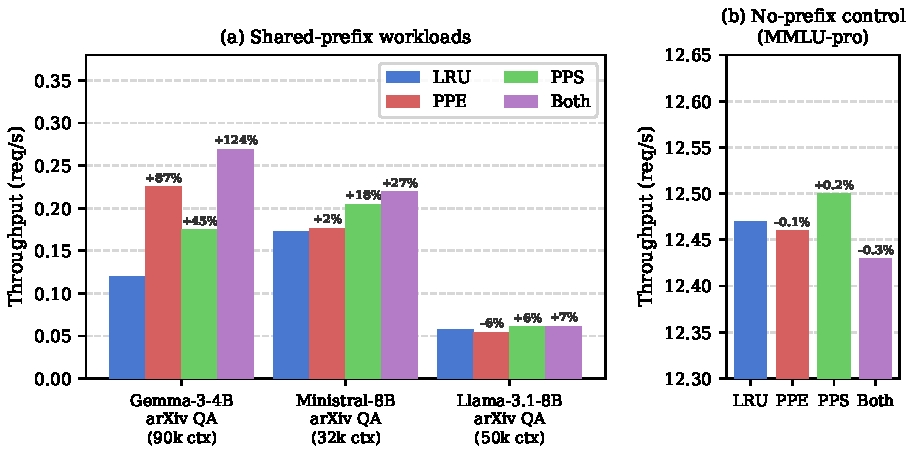
\includegraphics[width=\columnwidth]{figure1_throughput.pdf}
  \caption{Closed-loop throughput across models and workloads.
           (a) Three shared-prefix workloads; (b) MMLU-pro control (no shared
           prefix). All four policies lie within $\pm0.6\%$ of each other
           in~(b), confirming zero regression.}
  \label{fig:bar}
\end{figure}

\begin{table}[t]
\centering
\caption{Gemma-3-4B-IT — arXiv QA (90k avg.\ context, $\rho\approx5$).
Values are mean\,$\pm$\,std; $n$ = number of independent runs.}
\label{tab:gemma}
\renewcommand{\arraystretch}{1.2}
\begin{tabular}{@{}lcccc@{}}
\toprule
\textbf{Policy ($n$)} & \textbf{req/s} & \textbf{$\Delta$} &
\textbf{TTFT\textsubscript{mean} (s)} & \textbf{TTFT\textsubscript{p99} (s)} \\
\midrule
LRU (4)        & 0.126\,$\pm$\,.008 & ---     & 152\,$\pm$\,14 & 314\,$\pm$\,19 \\
\pps\ only (2) & 0.173\,$\pm$\,.003 & +37\%   & 100\,$\pm$\,2  & 227\,$\pm$\,4  \\
\ppe\ only (2) & 0.219\,$\pm$\,.009 & +74\%   &  94\,$\pm$\,2  & 179\,$\pm$\,9  \\
\textbf{Both (2)} & \textbf{0.267\,$\pm$\,.003} & \textbf{+112\%} &
                   \textbf{77\,$\pm$\,1} & \textbf{145\,$\pm$\,3} \\
\bottomrule
\end{tabular}
\end{table}

\begin{table}[t]
\centering
\caption{Ministral-8B FP8 — arXiv QA (32k avg.\ context, $\rho\approx2$).
Single run ($n=1$); variance data pending.}
\label{tab:ministral}
\renewcommand{\arraystretch}{1.2}
\begin{tabular}{@{}lcccc@{}}
\toprule
\textbf{Policy} & \textbf{req/s} & \textbf{$\Delta$} &
\textbf{TTFT\textsubscript{mean} (s)} & \textbf{TTFT\textsubscript{p99} (s)} \\
\midrule
LRU            & 0.1725 & ---     & 121.8 & 221.1 \\
\ppe\ only     & 0.1766 & +2.4\%  & 120.3 & 216.8 \\
\pps\ only     & 0.2044 & +18.5\% &  91.8 & 184.6 \\
\textbf{Both}  & \textbf{0.2193} & \textbf{+27.1\%} &
                 \textbf{87.6}  & \textbf{170.2} \\
\bottomrule
\end{tabular}
\end{table}

\begin{table}[t]
\centering
\caption{Llama-3.1-8B — arXiv QA (50k avg.\ context, $\rho\approx1.1$).
\ppe\ auto-disabled ($\rho<\rhomin$). Mean\,$\pm$\,std; $n$ per policy shown.}
\label{tab:llama}
\renewcommand{\arraystretch}{1.2}
\begin{tabular}{@{}lcccc@{}}
\toprule
\textbf{Policy ($n$)} & \textbf{req/s} & \textbf{$\Delta$} &
\textbf{TTFT\textsubscript{mean} (s)} & \textbf{TTFT\textsubscript{p99} (s)} \\
\midrule
LRU (4)        & 0.0578\,$\pm$\,.0006 & ---      & 341\,$\pm$\,8  & 679\,$\pm$\,7  \\
\ppe\ only (2) & 0.0557\,$\pm$\,.0020 & $-$3.6\% & 354\,$\pm$\,14 & 706\,$\pm$\,27 \\
\pps\ only (2) & 0.0630\,$\pm$\,.0032 & +9.0\%   & 294\,$\pm$\,11 & 630\,$\pm$\,33 \\
\textbf{Both (2)} & \textbf{0.0603\,$\pm$\,.0014} & \textbf{+4.3\%} &
                   \textbf{310\,$\pm$\,3} & \textbf{658\,$\pm$\,15} \\
\bottomrule
\end{tabular}
\end{table}

\begin{table}[t]
\centering
\caption{Llama-3.1-8B — MMLU-pro (4k context, no shared prefix).
Control: all policies within $\pm0.6\%$. LRU: $n=2$ (12.470\,$\pm$\,.003);
others: $n=1$.}
\label{tab:mmlu}
\renewcommand{\arraystretch}{1.2}
\begin{tabular}{@{}lcc@{}}
\toprule
\textbf{Policy} & \textbf{req/s} & \textbf{$\Delta$} \\
\midrule
LRU            & 12.47 & ---      \\
\ppe\ only     & 12.46 & $-$0.1\% \\
\pps\ only     & 12.50 & +0.3\%   \\
Both           & 12.43 & $-$0.3\% \\
\bottomrule
\end{tabular}
\end{table}

\textbf{Gemma-3-4B-IT ($\rho\approx5$, Table~\ref{tab:gemma}).}
With the pool holding approximately five articles simultaneously, \ppe\ is
highly effective: protecting a single article's blocks meaningfully extends
their lifetime and prevents costly re-prefills.  \ppe\ alone gains +74\%
throughput over the LRU mean; \pps\ alone gains +37\%.  The combined
configuration achieves +112\%, exceeding either mechanism individually.
Note that the LRU baseline has a run-to-run standard deviation of 6.4\%
(0.008\,req/s), which is large relative to the absolute throughput (0.126\,req/s)
and reflects GPU thermal variance at this very low serving rate.  Confidence in
the direction of improvement is high; confidence in the precise magnitude
requires additional runs. This compound gain arises because the two mechanisms
reinforce each other: \ppe\ keeps warm blocks alive across steps while \pps\
ensures those blocks are consumed at the earliest opportunity.

\textbf{Ministral-8B FP8 ($\rho\approx2$, Table~\ref{tab:ministral}).}
At $\rho=2$ the pool holds only two articles, limiting how many blocks \ppe\
can protect across steps.  \ppe\ accordingly provides only +2.4\%, while \pps\
continues to deliver +18.5\% by exploiting hit opportunities within each
scheduling step.  The combined configuration achieves +27.1\%, with \pps\ as
the dominant contributor.

\textbf{Llama-3.1-8B ($\rho\approx1.1$, Table~\ref{tab:llama}).}
The auto-disable condition $\rho<\rhomin=2.0$ fires; \ppe\ falls back to pure
LRU.  The \ppe-only row accordingly shows $-3.6\%$ (mean across 2 runs), which
is within the standard deviation of the LRU baseline and is not a meaningful
regression.  \pps\ contributes +9.0\% in mean throughput and reduces mean TTFT
by 14\%; the combined configuration achieves +4.3\%, slightly less than \pps\
alone, likely due to the interaction between a two-run \pps\ estimate and a
four-run LRU baseline.  The auto-disable is validated: the system avoids wasted
protection-set scanning in the low-$\rho$ regime.

\textbf{MMLU-pro control (Table~\ref{tab:mmlu}).}
All four policies produce throughput within $\pm0.6\%$ of LRU on independent
prompts with no shared prefix, confirming that both mechanisms impose
negligible overhead when prefix reuse is absent.

\subsection{Rate Sweep}
\label{sec:ratesweep}

Figure~\ref{fig:ratesweep} shows throughput, TTFT, and TPOT as a function of
Poisson request rate for Gemma-3-4B-IT (LRU vs.\ Both).

\begin{figure}[t]
  \centering
  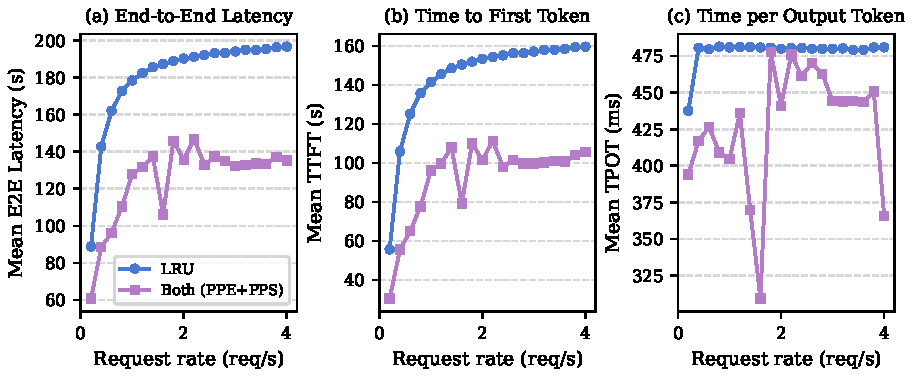
\includegraphics[width=\columnwidth]{figure2_rate_sweep.pdf}
  \caption{Gemma-3-4B-IT — Poisson rate sweep (0.2--4.0\,req/s, arXiv QA
           90k context, $n=1$ per rate point).  Both = \ppe{}+\pps\ combined;
           PPE-only and PPS-only curves are pending additional experiments.
           (a)~End-to-end latency; (b)~TTFT; (c)~TPOT.}
  \label{fig:ratesweep}
\end{figure}

\textbf{E2E Latency (Figure~\ref{fig:ratesweep}a).}
LRU E2EL grows monotonically from 89\,s at 0.2\,req/s to 197\,s at
4.0\,req/s as the queue deepens and every request waits behind a growing
prefill backlog.  Both compresses E2EL to 61--147\,s across the same range;
at rate$=$0.2 (lightly loaded) the reduction is 32\%; at rate$=$1.6 (peak
cache hit rate) it reaches 43\%.  The consistent gap reflects that higher
cache hit rates shorten per-request prefill time, reducing both queue wait
and compute latency.

\textbf{TTFT (Figure~\ref{fig:ratesweep}b).}
LRU TTFT grows monotonically with request rate (55\,s at 0.2\,req/s to
160\,s at 4.0\,req/s), reflecting an ever-deepening prefill queue.  Both TTFT
remains compressed (30--111\,s) because higher cache hit rates reduce
per-request prefill work, allowing queued requests to reach the decode phase
sooner.  The advantage over LRU ranges from 31\% to 46\% in mean TTFT.

\textbf{TPOT (Figure~\ref{fig:ratesweep}c).}
LRU TPOT locks at $\approx480$\,ms from rate $\geq0.4$.  The mechanism is
structural: in continuous batching~\cite{yu2022orca}, prefill tokens and decode
tokens share the same forward pass.  When every request requires a full
90k-token prefill, GPU compute is almost entirely consumed by prefill work,
and decode tokens are stalled waiting for their turn.  Both breaks this
bottleneck by reducing the prefill burden through higher cache hit rates: fewer
and shorter prefills leave more GPU bandwidth for decode, reducing per-token
latency.  The improvement ranges from 1\% to 36\% in mean TPOT, with the
largest gains occurring at rates where cache hit uplift is highest
(rate$=$1.6: 480\,ms $\to$ 309\,ms, $-$36\%).

At rates 1.8 and 2.2, Both TPOT reverts to near-LRU levels, coinciding with
lower-than-typical Both throughput at those rates.  A plausible cause is
batch-composition variance: at those specific rates, arrival-time jitter
may have yielded a higher fraction of cold-start requests in the batch.
Confirmation requires multiple seeds at those two rates, which we leave as
future work.

\subsection{Discussion}
\label{sec:discussion}

\textbf{\ppe\ effectiveness scales with $\rho$.}
The three closed-loop model configurations span $\rho\in\{1.1,2,5\}$, and
\ppe's mean benefit scales accordingly: +74\%, +2.4\%, and auto-disabled.
The pool ratio $\rho$ (Equation~\ref{eq:rho}) is a practical predictor of
\ppe\ utility: operators can estimate $\rho$ from model size, context length,
and GPU memory before enabling the mechanism.  The operating-regime boundary
$\rhomin=2.0$ is derived from three data points spanning distinct regimes;
it should be validated at intermediate values before being treated as a
precise threshold.

\textbf{\pps\ is broadly applicable.}
\pps\ provides mean gains of +37\%, +18.5\%, and +9.0\% across the three
pool regimes.  The diminishing returns at small $\rho$ are expected: when the
pool holds only one article, any scheduling order produces similar hit rates.
Nevertheless, even at $\rho\approx1.1$, \pps\ reduces mean TTFT by 14\%.

\textbf{Compound benefit at large $\rho$.}
The combined mean gain at $\rho\approx5$ (+112\%) exceeds either mechanism
alone.  This arises from a reinforcing interaction: \ppe\ preserves warm
blocks across steps; \pps\ directs the right requests to those blocks within
each step.  Both mechanisms must be active for this interaction to occur.

\textbf{Zero regression on non-prefix workloads.}
The MMLU-pro result confirms both mechanisms are safe to enable
unconditionally: they add no measurable overhead when prefix reuse is absent.

\subsection{Limitations}
\label{sec:limitations}

The following gaps constrain the strength of the current conclusions and
motivate future work:

\textbf{Rate sweep covers only one model and two policies.}
Figure~\ref{fig:ratesweep} shows only LRU and Both for Gemma-3-4B-IT.
Individual PPE-only and PPS-only rate-sweep curves are not available, so we
cannot isolate each mechanism's contribution under open-loop conditions.
Similarly, rate sweeps for Ministral-8B FP8 and Llama-3.1-8B are absent.

\textbf{Single GPU platform.}
All experiments use an A5000 (24\,GB).  On H100 (80\,GB), $\rho$ for the same
Gemma model would reach $\approx15$--20, potentially amplifying \ppe\ gains
further; on L4 (24\,GB), results would be similar to the A5000.

\textbf{Statistical coverage.}  Ministral results are single-run; all
closed-loop results have $n\leq4$.  The LRU baseline for Gemma shows 6.4\%
run-to-run variance, which limits precision of the reported $\Delta$ values.

\textbf{Cache hit rate not directly measured.}  The primary outcome of both
mechanisms is an increase in effective prefix cache hit rate, yet this metric
is not reported.  Including it in future experiments would provide a direct
mechanistic link between the policy change and the latency/throughput outcomes.

% ---------------------------------------------------------------
\section{Related Work}
\label{sec:related}
% ---------------------------------------------------------------

\textbf{LLM serving systems.}
vLLM~\cite{kwon2023efficient} introduced paged attention and block-level KV
management.  Orca~\cite{yu2022orca} proposed continuous batching to improve
decoding throughput.  Sarathi-Serve~\cite{agrawal2024sarathi} addresses
chunked prefill to reduce prefill-induced latency spikes.
FlashAttention~\cite{dao2022flashattention} provides the efficient attention
kernel that underlies modern LLM serving.
DistServe~\cite{zhong2024distserve} disaggregates prefill and decode phases
onto separate GPU pools to reduce their mutual interference—a problem that our
TPOT analysis (Section~\ref{sec:ratesweep}) highlights as central to the
benefit of reducing prefill work via cache hits.
Our work is orthogonal to all of these: we improve the scheduling and
eviction subsystems without modifying attention kernels or batch formation
logic.

\textbf{Prefix caching and long-context serving.}
SGLang~\cite{zheng2023sglang} introduced RadixAttention, which organises the
KV cache as a radix tree to enable efficient prefix sharing across requests
with variable-length common prefixes.  ChunkAttention~\cite{ye2024chunkattention}
exploits prefix structure at the attention computation level to share KV blocks
across concurrent sequences.  Hydragen~\cite{juravsky2024hydragen} batches
the shared-prefix attention computation across multiple requests to improve GPU
utilisation, which is complementary to our eviction and scheduling approach.
Mooncake~\cite{qin2024mooncake} proposes KV cache disaggregation with
prefix-aware routing across machines; our work addresses the single-node case,
which arises both independently and as the local-node component of disaggregated
deployments.

\textbf{KV cache eviction.}
MemServe~\cite{hu2024memserve} studies KV cache lifetime management at cluster
scale.  CacheBlend~\cite{yao2024cacheblend} proposes selective recomputation
of cross-attention blocks during prefix reuse, trading computation for
freshness.  InfiniGen~\cite{gim2024infinigen} reduces KV memory pressure via
dynamic eviction of speculative future tokens, complementing our approach of
protecting blocks for \emph{known} pending requests.
Our \ppe\ addresses a complementary, within-node problem: the LRU policy's
blindness to the waiting queue.  It can be combined with any of the above
placement strategies.

\textbf{Scheduler-aware prefix management.}
Preble~\cite{shi2024preble} co-designs scheduling and caching for multi-GPU
prefix routing, assigning requests to the GPU that already holds the relevant
prefix.  Our \pps\ addresses the simpler but important single-node case, where
the scheduler and KV cache share address space and prefix inspection is cheap
and read-only.
BatchLLM~\cite{zheng2024batchllm} identifies and groups requests with shared
prefixes to form prefix-optimised batches; our \pps\ achieves a similar
grouping effect dynamically through priority-ordered scheduling without
requiring explicit prefix clustering.

\textbf{Jenga.}
\jenga~\cite{jenga2025} is the base system for our implementation.  It decides
\emph{where} blocks reside across GPU/CPU/NVMe; \ppe\ decides \emph{which}
free GPU blocks survive eviction; \pps\ decides \emph{which} requests are
served first.  The three concerns are fully orthogonal, and our mechanisms are
compatible with all three \jenga\ allocator policies.

% ---------------------------------------------------------------
\section{Conclusion}
\label{sec:conc}
% ---------------------------------------------------------------

We presented Prefix Peeking Eviction (\ppe) and Prefix Peeking Scheduling
(\pps), two demand-aware, opt-in extensions for LLM serving built on top of
\jenga.  \ppe\ inspects the waiting queue before each scheduling step and
protects the free KV cache blocks that queued requests will immediately reuse,
preventing LRU from evicting them.  A budget cap and a pool-size auto-disable
heuristic bound overhead and prevent degradation in low-$\rho$ regimes.
\pps\ prioritises cache-warm requests via a lazy priority sort with an
anti-starvation guarantee.

Closed-loop experiments across three models confirm that the combined system
achieves a mean of $2.12\times$ higher throughput and 49\% lower mean TTFT over
LRU on Gemma-3-4B-IT ($\rho\approx5$, $n=2$--$4$ runs).  The
pool-size-to-article-size ratio~$\rho$ serves as an operating-regime indicator
for \ppe\ utility; \pps\ provides consistent gains regardless of $\rho$.  A
Poisson rate-sweep over 20 operating points confirms Both outperforms LRU by
25--81\% in throughput and 20--46\% in E2E latency across the full load range,
with TPOT improvements of up to 36\% attributable to reduced per-step prefill
work.  A MMLU-pro control experiment confirms $<0.6\%$ throughput variance on
workloads without shared prefixes.

Future work includes: (1) adding PPE-only and PPS-only curves to the rate
sweep, and extending the sweep to Ministral-8B FP8 and Llama-3.1-8B; (2)
evaluating on H100 and L4 GPUs to align with the \jenga\ baseline
platform~\cite{jenga2025} and cover higher $\rho$ regimes; (3) reporting
prefix cache hit rate as a direct metric linking policy changes to
latency/throughput outcomes; (4) studying the interaction between \ppe\ and
\jenga's CPU/NVMe eviction tiers under memory pressure; (5) deriving an
analytical formulation of $\rhomin$ grounded in eviction miss-rate models; and
(6) adapting the protection budget cap dynamically using online telemetry.

% ---------------------------------------------------------------
\bibliographystyle{IEEEtran}

\begin{thebibliography}{14}

\bibitem{jenga2025}
[Authors],
``Jenga: Effective Memory Management for Serving LLM with Heterogeneity,''
in \emph{Proc.\ ACM Symp.\ Operating Systems Principles (SOSP)}, 2025.

\bibitem{kwon2023efficient}
W.~Kwon \emph{et al.},
``Efficient Memory Management for Large Language Model Serving with
PagedAttention,''
in \emph{Proc.\ ACM SOSP}, 2023.

\bibitem{yu2022orca}
G.~Yu \emph{et al.},
``Orca: A Distributed Serving System for Transformer-Based Generative Models,''
in \emph{Proc.\ USENIX OSDI}, 2022.

\bibitem{agrawal2024sarathi}
A.~Agrawal \emph{et al.},
``Sarathi-Serve: Efficient LLM Serving by Piggybacking Decodes with Chunked
Prefills,''
in \emph{Proc.\ USENIX OSDI}, 2024.

\bibitem{dao2022flashattention}
T.~Dao, D.~Fu, S.~Ermon, A.~Rudra, and C.~R{\'e},
``FlashAttention: Fast and Memory-Efficient Exact Attention with IO-Awareness,''
in \emph{Advances in Neural Information Processing Systems (NeurIPS)}, 2022.

\bibitem{zhong2024distserve}
Y.~Zhong \emph{et al.},
``DistServe: Disaggregating Prefill and Decoding for Goodput-Optimized Large
Language Model Serving,''
in \emph{Proc.\ USENIX OSDI}, 2024.

\bibitem{zheng2023sglang}
L.~Zheng \emph{et al.},
``Efficiently Programming Large Language Models using SGLang,''
\emph{arXiv:2312.07104}, 2023.

\bibitem{ye2024chunkattention}
M.~Ye, T.~Xu, G.~Lai, and X.~Liu,
``ChunkAttention: Efficient Self-Attention with Prefix-Aware KV Cache and
Two-Phase Partition,''
\emph{arXiv:2402.15220}, 2024.

\bibitem{juravsky2024hydragen}
J.~Juravsky \emph{et al.},
``Hydragen: High-Throughput LLM Inference with Shared Prefixes,''
\emph{arXiv:2402.05099}, 2024.

\bibitem{qin2024mooncake}
R.~Qin \emph{et al.},
``Mooncake: A KVCache-centric Disaggregated Architecture for LLM Serving,''
\emph{arXiv:2407.00079}, 2024.

\bibitem{hu2024memserve}
Y.~Hu \emph{et al.},
``MemServe: Context Caching for Disaggregated LLM Serving with Elastic Memory
Pool,''
\emph{arXiv:2406.17565}, 2024.

\bibitem{yao2024cacheblend}
J.~Yao \emph{et al.},
``CacheBlend: Fast Large Language Model Serving for RAG with Cached Knowledge
Fusion,''
\emph{arXiv:2405.16444}, 2024.

\bibitem{shi2024preble}
Y.~Shi \emph{et al.},
``Preble: Efficient Distributed Prompt Scheduling for LLM Serving,''
\emph{arXiv:2407.00023}, 2024.

\bibitem{gim2024infinigen}
J.~Gim \emph{et al.},
``InfiniGen: Efficient Generative Inference of Large Language Models with
Dynamic KV Cache Management,''
in \emph{Proc.\ USENIX OSDI}, 2024.

\bibitem{zheng2024batchllm}
Z.~Zheng \emph{et al.},
``BatchLLM: Optimizing Large Batched LLM Inference with Global Prefix Sharing
and Throughput-oriented Token Batching,''
\emph{arXiv:2412.03594}, 2024.

\end{thebibliography}

\balance
\end{document}
